\documentclass[12pt]{article}
\usepackage{tikz}
\usepackage{amsmath}
% Underlining package
\usepackage{ulem}
\usepackage[a4paper, portrait, margin=1cm]{geometry}
\usepackage{fancyhdr}

\def \HeadingAnswers {\section*{\Large Name: \underline{\hspace{8cm}} \hfill Date: \underline{\hspace{3cm}}} \vspace{-3mm}
{Levers: Answers} \vspace{1pt}\hrule}

% raise footer with page number; no header
\fancypagestyle{myfancypagestyle}{
  \fancyhf{}% clear all header and footer fields
  \renewcommand{\headrulewidth}{0pt} % no rule under header
  \fancyfoot[C] {\thepage} \setlength{\footskip}{6pt} % raise page number 6pt
}
\pagestyle{myfancypagestyle}  % apply myfancypagestyle

\newcounter{minipagecount}

\begin{document}
\HeadingAnswers
\vspace{8mm}

\refstepcounter{minipagecount}
\noindent{(\theminipagecount)}\quad

\begin{minipage}{0.65\textwidth}
    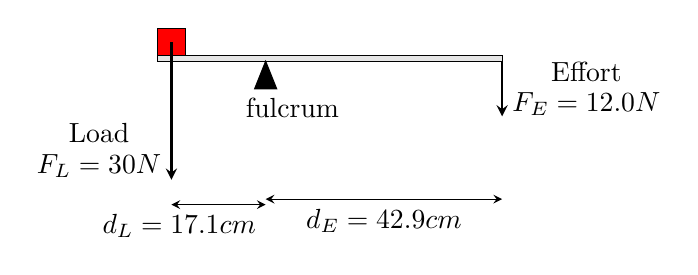
\begin{tikzpicture}[scale=0.7,>=stealth]
        % First class lever
        % rod
        \draw[fill=gray!20] (-0.25,0) rectangle (6,0.1);
        %fulcrum
        \draw[fill=black] (1.51,-0.5) -- (1.91,-0.5) node[below,xshift=2mm] {fulcrum} -- (1.71,0) -- cycle;
        %load
        \draw[fill=red] (-0.25,0.1) rectangle (0.25,0.6);
        \draw[->,thick] (0.0,0.35) -- (0.0,-2.15) node[midway,left,yshift=-0.5cm,align=center] {Load \\\\[-3ex] $F_L = 30N$};
        %effort
        \draw[->,thick] (6,0.0) -- (6,-1.0) node[midway,right,align=center] {Effort \\\\[-3ex] $F_E = 12.0N$};

        % Distance markers
        \draw[<->] (1.71,-2.5) -- (6,-2.5) node[midway,below,align=center] {$d_E = 42.9cm$};
        \draw[<->] (0,-2.6) -- (1.71,-2.6) node[midway,below,xshift=-0.5cm,align=left] {$d_L = 17.1cm$};
    \end{tikzpicture}
\end{minipage}%
\hfill
\begin{minipage}{0.3\textwidth}
    \begin{align*}
        F_E \times d_E &= F_L \times d_L \\
        F_E &= \frac{F_L \times d_L}{d_E} \\
        F_E &= \frac{30 \times 17.1}{42.9} \\
        F_E &= 12.0N
    \end{align*}
\end{minipage}
\refstepcounter{minipagecount}
\noindent{(\theminipagecount)}\quad

\begin{minipage}{0.65\textwidth}
    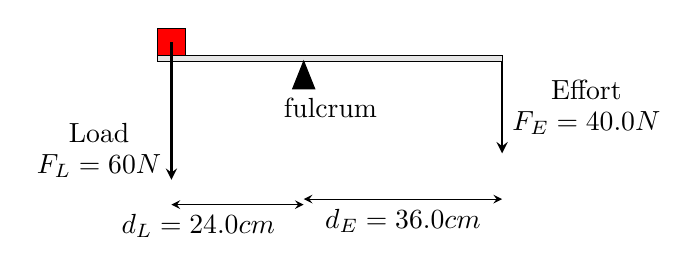
\begin{tikzpicture}[scale=0.7,>=stealth]
        % First class lever
        % rod
        \draw[fill=gray!20] (-0.25,0) rectangle (6,0.1);
        %fulcrum
        \draw[fill=black] (2.2,-0.5) -- (2.6,-0.5) node[below,xshift=2mm] {fulcrum} -- (2.4,0) -- cycle;
        %load
        \draw[fill=red] (-0.25,0.1) rectangle (0.25,0.6);
        \draw[->,thick] (0.0,0.35) -- (0.0,-2.15) node[midway,left,yshift=-0.5cm,align=center] {Load \\\\[-3ex] $F_L = 60N$};
        %effort
        \draw[->,thick] (6,0.0) -- (6,-1.67) node[midway,right,align=center] {Effort \\\\[-3ex] $F_E = 40.0N$};

        % Distance markers
        \draw[<->] (2.4,-2.5) -- (6,-2.5) node[midway,below,align=center] {$d_E = 36.0cm$};
        \draw[<->] (0,-2.6) -- (2.4,-2.6) node[midway,below,xshift=-0.5cm,align=left] {$d_L = 24.0cm$};
    \end{tikzpicture}
\end{minipage}%
\hfill
\begin{minipage}{0.3\textwidth}
    \begin{align*}
        F_E \times d_E &= F_L \times d_L \\
        F_E &= \frac{F_L \times d_L}{d_E} \\
        F_E &= \frac{60 \times 24.0}{36.0} \\
        F_E &= 40.0N
    \end{align*}
\end{minipage}
\refstepcounter{minipagecount}
\noindent{(\theminipagecount)}\quad

\begin{minipage}{0.65\textwidth}
    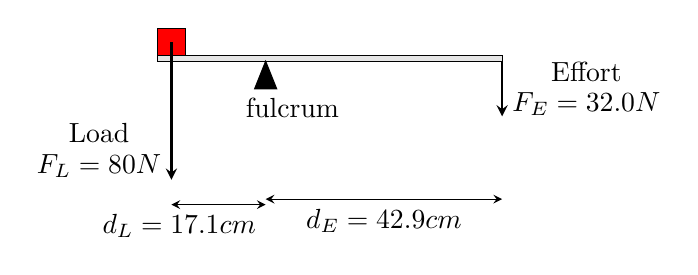
\begin{tikzpicture}[scale=0.7,>=stealth]
        % First class lever
        % rod
        \draw[fill=gray!20] (-0.25,0) rectangle (6,0.1);
        %fulcrum
        \draw[fill=black] (1.51,-0.5) -- (1.91,-0.5) node[below,xshift=2mm] {fulcrum} -- (1.71,0) -- cycle;
        %load
        \draw[fill=red] (-0.25,0.1) rectangle (0.25,0.6);
        \draw[->,thick] (0.0,0.35) -- (0.0,-2.15) node[midway,left,yshift=-0.5cm,align=center] {Load \\\\[-3ex] $F_L = 80N$};
        %effort
        \draw[->,thick] (6,0.0) -- (6,-1.0) node[midway,right,align=center] {Effort \\\\[-3ex] $F_E = 32.0N$};

        % Distance markers
        \draw[<->] (1.71,-2.5) -- (6,-2.5) node[midway,below,align=center] {$d_E = 42.9cm$};
        \draw[<->] (0,-2.6) -- (1.71,-2.6) node[midway,below,xshift=-0.5cm,align=left] {$d_L = 17.1cm$};
    \end{tikzpicture}
\end{minipage}%
\hfill
\begin{minipage}{0.3\textwidth}
    \begin{align*}
        F_E \times d_E &= F_L \times d_L \\
        F_E &= \frac{F_L \times d_L}{d_E} \\
        F_E &= \frac{80 \times 17.1}{42.9} \\
        F_E &= 32.0N
    \end{align*}
\end{minipage}
\refstepcounter{minipagecount}
\noindent{(\theminipagecount)}\quad

\begin{minipage}{0.65\textwidth}
    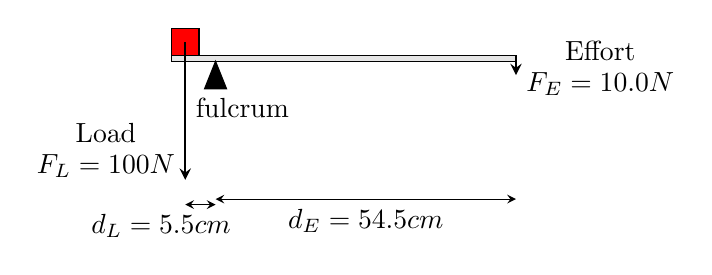
\begin{tikzpicture}[scale=0.7,>=stealth]
        % First class lever
        % rod
        \draw[fill=gray!20] (-0.25,0) rectangle (6,0.1);
        %fulcrum
        \draw[fill=black] (0.35,-0.5) -- (0.75,-0.5) node[below,xshift=2mm] {fulcrum} -- (0.55,0) -- cycle;
        %load
        \draw[fill=red] (-0.25,0.1) rectangle (0.25,0.6);
        \draw[->,thick] (0.0,0.35) -- (0.0,-2.15) node[midway,left,yshift=-0.5cm,align=center] {Load \\\\[-3ex] $F_L = 100N$};
        %effort
        \draw[->,thick] (6,0.0) -- (6,-0.25) node[midway,right,align=center] {Effort \\\\[-3ex] $F_E = 10.0N$};

        % Distance markers
        \draw[<->] (0.55,-2.5) -- (6,-2.5) node[midway,below,align=center] {$d_E = 54.5cm$};
        \draw[<->] (0,-2.6) -- (0.55,-2.6) node[midway,below,xshift=-0.5cm,align=left] {$d_L = 5.5cm$};
    \end{tikzpicture}
\end{minipage}%
\hfill
\begin{minipage}{0.3\textwidth}
    \begin{align*}
        F_E \times d_E &= F_L \times d_L \\
        F_E &= \frac{F_L \times d_L}{d_E} \\
        F_E &= \frac{100 \times 5.5}{54.5} \\
        F_E &= 10.0N
    \end{align*}
\end{minipage}
\refstepcounter{minipagecount}
\noindent{(\theminipagecount)}\quad

\begin{minipage}{0.65\textwidth}
    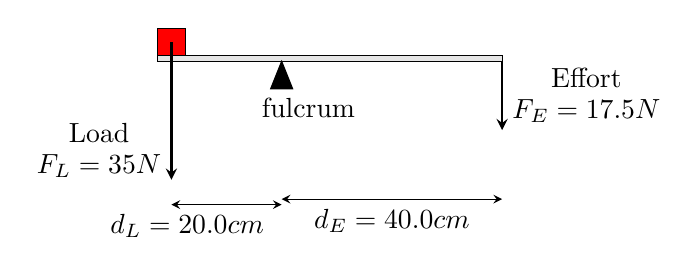
\begin{tikzpicture}[scale=0.7,>=stealth]
        % First class lever
        % rod
        \draw[fill=gray!20] (-0.25,0) rectangle (6,0.1);
        %fulcrum
        \draw[fill=black] (1.8,-0.5) -- (2.2,-0.5) node[below,xshift=2mm] {fulcrum} -- (2.0,0) -- cycle;
        %load
        \draw[fill=red] (-0.25,0.1) rectangle (0.25,0.6);
        \draw[->,thick] (0.0,0.35) -- (0.0,-2.15) node[midway,left,yshift=-0.5cm,align=center] {Load \\\\[-3ex] $F_L = 35N$};
        %effort
        \draw[->,thick] (6,0.0) -- (6,-1.25) node[midway,right,align=center] {Effort \\\\[-3ex] $F_E = 17.5N$};

        % Distance markers
        \draw[<->] (2.0,-2.5) -- (6,-2.5) node[midway,below,align=center] {$d_E = 40.0cm$};
        \draw[<->] (0,-2.6) -- (2.0,-2.6) node[midway,below,xshift=-0.5cm,align=left] {$d_L = 20.0cm$};
    \end{tikzpicture}
\end{minipage}%
\hfill
\begin{minipage}{0.3\textwidth}
    \begin{align*}
        F_E \times d_E &= F_L \times d_L \\
        F_E &= \frac{F_L \times d_L}{d_E} \\
        F_E &= \frac{35 \times 20.0}{40.0} \\
        F_E &= 17.5N
    \end{align*}
\end{minipage}
\pagebreak ~ \newline ~ \newline\refstepcounter{minipagecount}
\noindent{(\theminipagecount)}\quad

\begin{minipage}{0.65\textwidth}
    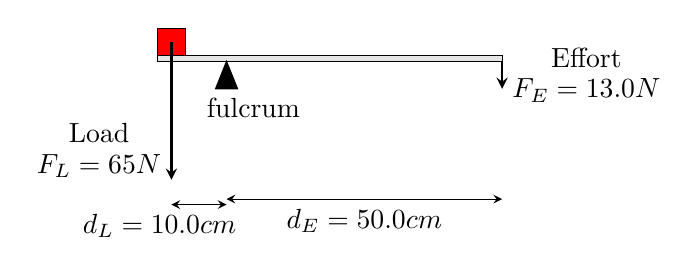
\begin{tikzpicture}[scale=0.7,>=stealth]
        % First class lever
        % rod
        \draw[fill=gray!20] (-0.25,0) rectangle (6,0.1);
        %fulcrum
        \draw[fill=black] (0.8,-0.5) -- (1.2,-0.5) node[below,xshift=2mm] {fulcrum} -- (1.0,0) -- cycle;
        %load
        \draw[fill=red] (-0.25,0.1) rectangle (0.25,0.6);
        \draw[->,thick] (0.0,0.35) -- (0.0,-2.15) node[midway,left,yshift=-0.5cm,align=center] {Load \\\\[-3ex] $F_L = 65N$};
        %effort
        \draw[->,thick] (6,0.0) -- (6,-0.5) node[midway,right,align=center] {Effort \\\\[-3ex] $F_E = 13.0N$};

        % Distance markers
        \draw[<->] (1.0,-2.5) -- (6,-2.5) node[midway,below,align=center] {$d_E = 50.0cm$};
        \draw[<->] (0,-2.6) -- (1.0,-2.6) node[midway,below,xshift=-0.5cm,align=left] {$d_L = 10.0cm$};
    \end{tikzpicture}
\end{minipage}%
\hfill
\begin{minipage}{0.3\textwidth}
    \begin{align*}
        F_E \times d_E &= F_L \times d_L \\
        F_E &= \frac{F_L \times d_L}{d_E} \\
        F_E &= \frac{65 \times 10.0}{50.0} \\
        F_E &= 13.0N
    \end{align*}
\end{minipage}
\refstepcounter{minipagecount}
\noindent{(\theminipagecount)}\quad

\begin{minipage}{0.65\textwidth}
    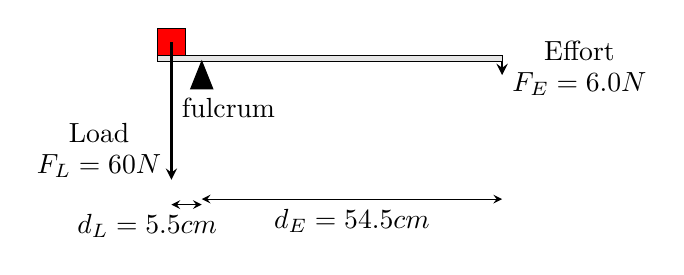
\begin{tikzpicture}[scale=0.7,>=stealth]
        % First class lever
        % rod
        \draw[fill=gray!20] (-0.25,0) rectangle (6,0.1);
        %fulcrum
        \draw[fill=black] (0.35,-0.5) -- (0.75,-0.5) node[below,xshift=2mm] {fulcrum} -- (0.55,0) -- cycle;
        %load
        \draw[fill=red] (-0.25,0.1) rectangle (0.25,0.6);
        \draw[->,thick] (0.0,0.35) -- (0.0,-2.15) node[midway,left,yshift=-0.5cm,align=center] {Load \\\\[-3ex] $F_L = 60N$};
        %effort
        \draw[->,thick] (6,0.0) -- (6,-0.25) node[midway,right,align=center] {Effort \\\\[-3ex] $F_E = 6.0N$};

        % Distance markers
        \draw[<->] (0.55,-2.5) -- (6,-2.5) node[midway,below,align=center] {$d_E = 54.5cm$};
        \draw[<->] (0,-2.6) -- (0.55,-2.6) node[midway,below,xshift=-0.5cm,align=left] {$d_L = 5.5cm$};
    \end{tikzpicture}
\end{minipage}%
\hfill
\begin{minipage}{0.3\textwidth}
    \begin{align*}
        F_E \times d_E &= F_L \times d_L \\
        F_E &= \frac{F_L \times d_L}{d_E} \\
        F_E &= \frac{60 \times 5.5}{54.5} \\
        F_E &= 6.0N
    \end{align*}
\end{minipage}
\refstepcounter{minipagecount}
\noindent{(\theminipagecount)}\quad

\begin{minipage}{0.65\textwidth}
    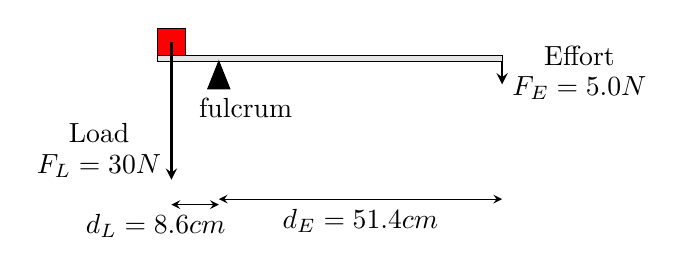
\begin{tikzpicture}[scale=0.7,>=stealth]
        % First class lever
        % rod
        \draw[fill=gray!20] (-0.25,0) rectangle (6,0.1);
        %fulcrum
        \draw[fill=black] (0.66,-0.5) -- (1.06,-0.5) node[below,xshift=2mm] {fulcrum} -- (0.86,0) -- cycle;
        %load
        \draw[fill=red] (-0.25,0.1) rectangle (0.25,0.6);
        \draw[->,thick] (0.0,0.35) -- (0.0,-2.15) node[midway,left,yshift=-0.5cm,align=center] {Load \\\\[-3ex] $F_L = 30N$};
        %effort
        \draw[->,thick] (6,0.0) -- (6,-0.42) node[midway,right,align=center] {Effort \\\\[-3ex] $F_E = 5.0N$};

        % Distance markers
        \draw[<->] (0.86,-2.5) -- (6,-2.5) node[midway,below,align=center] {$d_E = 51.4cm$};
        \draw[<->] (0,-2.6) -- (0.86,-2.6) node[midway,below,xshift=-0.5cm,align=left] {$d_L = 8.6cm$};
    \end{tikzpicture}
\end{minipage}%
\hfill
\begin{minipage}{0.3\textwidth}
    \begin{align*}
        F_E \times d_E &= F_L \times d_L \\
        F_E &= \frac{F_L \times d_L}{d_E} \\
        F_E &= \frac{30 \times 8.6}{51.4} \\
        F_E &= 5.0N
    \end{align*}
\end{minipage}
\refstepcounter{minipagecount}
\noindent{(\theminipagecount)}\quad

\begin{minipage}{0.65\textwidth}
    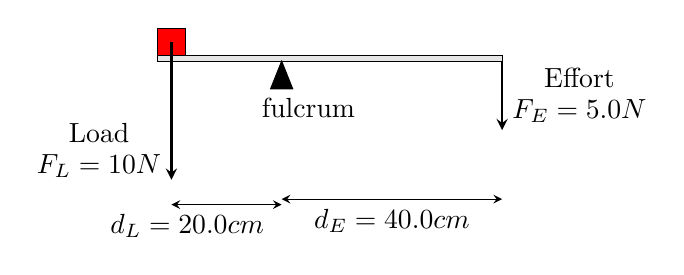
\begin{tikzpicture}[scale=0.7,>=stealth]
        % First class lever
        % rod
        \draw[fill=gray!20] (-0.25,0) rectangle (6,0.1);
        %fulcrum
        \draw[fill=black] (1.8,-0.5) -- (2.2,-0.5) node[below,xshift=2mm] {fulcrum} -- (2.0,0) -- cycle;
        %load
        \draw[fill=red] (-0.25,0.1) rectangle (0.25,0.6);
        \draw[->,thick] (0.0,0.35) -- (0.0,-2.15) node[midway,left,yshift=-0.5cm,align=center] {Load \\\\[-3ex] $F_L = 10N$};
        %effort
        \draw[->,thick] (6,0.0) -- (6,-1.25) node[midway,right,align=center] {Effort \\\\[-3ex] $F_E = 5.0N$};

        % Distance markers
        \draw[<->] (2.0,-2.5) -- (6,-2.5) node[midway,below,align=center] {$d_E = 40.0cm$};
        \draw[<->] (0,-2.6) -- (2.0,-2.6) node[midway,below,xshift=-0.5cm,align=left] {$d_L = 20.0cm$};
    \end{tikzpicture}
\end{minipage}%
\hfill
\begin{minipage}{0.3\textwidth}
    \begin{align*}
        F_E \times d_E &= F_L \times d_L \\
        F_E &= \frac{F_L \times d_L}{d_E} \\
        F_E &= \frac{10 \times 20.0}{40.0} \\
        F_E &= 5.0N
    \end{align*}
\end{minipage}
\refstepcounter{minipagecount}
\noindent{(\theminipagecount)}\quad

\begin{minipage}{0.65\textwidth}
    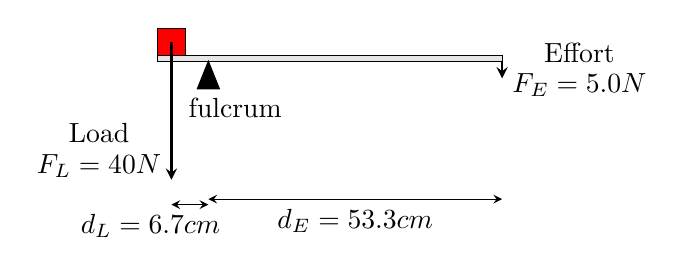
\begin{tikzpicture}[scale=0.7,>=stealth]
        % First class lever
        % rod
        \draw[fill=gray!20] (-0.25,0) rectangle (6,0.1);
        %fulcrum
        \draw[fill=black] (0.47,-0.5) -- (0.87,-0.5) node[below,xshift=2mm] {fulcrum} -- (0.67,0) -- cycle;
        %load
        \draw[fill=red] (-0.25,0.1) rectangle (0.25,0.6);
        \draw[->,thick] (0.0,0.35) -- (0.0,-2.15) node[midway,left,yshift=-0.5cm,align=center] {Load \\\\[-3ex] $F_L = 40N$};
        %effort
        \draw[->,thick] (6,0.0) -- (6,-0.31) node[midway,right,align=center] {Effort \\\\[-3ex] $F_E = 5.0N$};

        % Distance markers
        \draw[<->] (0.67,-2.5) -- (6,-2.5) node[midway,below,align=center] {$d_E = 53.3cm$};
        \draw[<->] (0,-2.6) -- (0.67,-2.6) node[midway,below,xshift=-0.5cm,align=left] {$d_L = 6.7cm$};
    \end{tikzpicture}
\end{minipage}%
\hfill
\begin{minipage}{0.3\textwidth}
    \begin{align*}
        F_E \times d_E &= F_L \times d_L \\
        F_E &= \frac{F_L \times d_L}{d_E} \\
        F_E &= \frac{40 \times 6.7}{53.3} \\
        F_E &= 5.0N
    \end{align*}
\end{minipage}
\pagebreak ~ \newline ~ \newline\refstepcounter{minipagecount}
\noindent{(\theminipagecount)}\quad

\begin{minipage}{0.65\textwidth}
    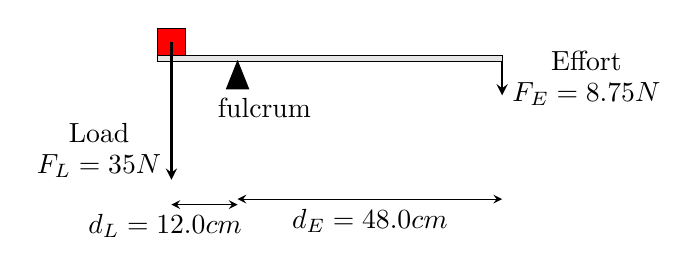
\begin{tikzpicture}[scale=0.7,>=stealth]
        % First class lever
        % rod
        \draw[fill=gray!20] (-0.25,0) rectangle (6,0.1);
        %fulcrum
        \draw[fill=black] (1.0,-0.5) -- (1.4,-0.5) node[below,xshift=2mm] {fulcrum} -- (1.2,0) -- cycle;
        %load
        \draw[fill=red] (-0.25,0.1) rectangle (0.25,0.6);
        \draw[->,thick] (0.0,0.35) -- (0.0,-2.15) node[midway,left,yshift=-0.5cm,align=center] {Load \\\\[-3ex] $F_L = 35N$};
        %effort
        \draw[->,thick] (6,0.0) -- (6,-0.62) node[midway,right,align=center] {Effort \\\\[-3ex] $F_E = 8.75N$};

        % Distance markers
        \draw[<->] (1.2,-2.5) -- (6,-2.5) node[midway,below,align=center] {$d_E = 48.0cm$};
        \draw[<->] (0,-2.6) -- (1.2,-2.6) node[midway,below,xshift=-0.5cm,align=left] {$d_L = 12.0cm$};
    \end{tikzpicture}
\end{minipage}%
\hfill
\begin{minipage}{0.3\textwidth}
    \begin{align*}
        F_E \times d_E &= F_L \times d_L \\
        F_E &= \frac{F_L \times d_L}{d_E} \\
        F_E &= \frac{35 \times 12.0}{48.0} \\
        F_E &= 8.75N
    \end{align*}
\end{minipage}
\refstepcounter{minipagecount}
\noindent{(\theminipagecount)}\quad

\begin{minipage}{0.65\textwidth}
    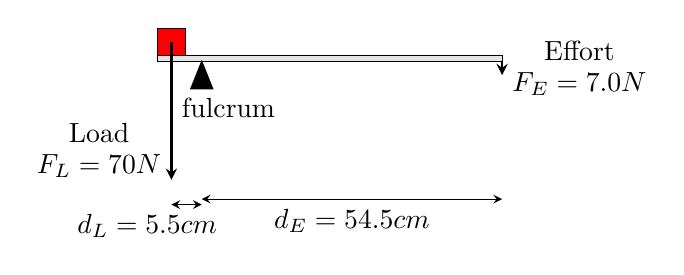
\begin{tikzpicture}[scale=0.7,>=stealth]
        % First class lever
        % rod
        \draw[fill=gray!20] (-0.25,0) rectangle (6,0.1);
        %fulcrum
        \draw[fill=black] (0.35,-0.5) -- (0.75,-0.5) node[below,xshift=2mm] {fulcrum} -- (0.55,0) -- cycle;
        %load
        \draw[fill=red] (-0.25,0.1) rectangle (0.25,0.6);
        \draw[->,thick] (0.0,0.35) -- (0.0,-2.15) node[midway,left,yshift=-0.5cm,align=center] {Load \\\\[-3ex] $F_L = 70N$};
        %effort
        \draw[->,thick] (6,0.0) -- (6,-0.25) node[midway,right,align=center] {Effort \\\\[-3ex] $F_E = 7.0N$};

        % Distance markers
        \draw[<->] (0.55,-2.5) -- (6,-2.5) node[midway,below,align=center] {$d_E = 54.5cm$};
        \draw[<->] (0,-2.6) -- (0.55,-2.6) node[midway,below,xshift=-0.5cm,align=left] {$d_L = 5.5cm$};
    \end{tikzpicture}
\end{minipage}%
\hfill
\begin{minipage}{0.3\textwidth}
    \begin{align*}
        F_E \times d_E &= F_L \times d_L \\
        F_E &= \frac{F_L \times d_L}{d_E} \\
        F_E &= \frac{70 \times 5.5}{54.5} \\
        F_E &= 7.0N
    \end{align*}
\end{minipage}
\refstepcounter{minipagecount}
\noindent{(\theminipagecount)}\quad

\begin{minipage}{0.65\textwidth}
    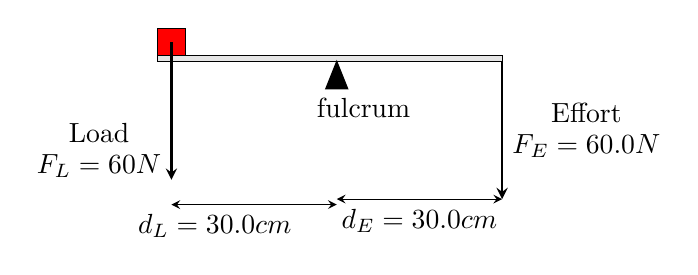
\begin{tikzpicture}[scale=0.7,>=stealth]
        % First class lever
        % rod
        \draw[fill=gray!20] (-0.25,0) rectangle (6,0.1);
        %fulcrum
        \draw[fill=black] (2.8,-0.5) -- (3.2,-0.5) node[below,xshift=2mm] {fulcrum} -- (3.0,0) -- cycle;
        %load
        \draw[fill=red] (-0.25,0.1) rectangle (0.25,0.6);
        \draw[->,thick] (0.0,0.35) -- (0.0,-2.15) node[midway,left,yshift=-0.5cm,align=center] {Load \\\\[-3ex] $F_L = 60N$};
        %effort
        \draw[->,thick] (6,0.0) -- (6,-2.5) node[midway,right,align=center] {Effort \\\\[-3ex] $F_E = 60.0N$};

        % Distance markers
        \draw[<->] (3.0,-2.5) -- (6,-2.5) node[midway,below,align=center] {$d_E = 30.0cm$};
        \draw[<->] (0,-2.6) -- (3.0,-2.6) node[midway,below,xshift=-0.5cm,align=left] {$d_L = 30.0cm$};
    \end{tikzpicture}
\end{minipage}%
\hfill
\begin{minipage}{0.3\textwidth}
    \begin{align*}
        F_E \times d_E &= F_L \times d_L \\
        F_E &= \frac{F_L \times d_L}{d_E} \\
        F_E &= \frac{60 \times 30.0}{30.0} \\
        F_E &= 60.0N
    \end{align*}
\end{minipage}
\refstepcounter{minipagecount}
\noindent{(\theminipagecount)}\quad

\begin{minipage}{0.65\textwidth}
    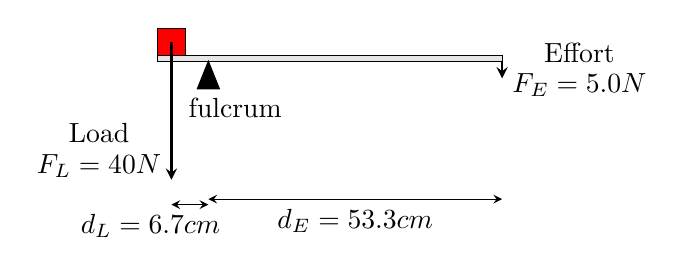
\begin{tikzpicture}[scale=0.7,>=stealth]
        % First class lever
        % rod
        \draw[fill=gray!20] (-0.25,0) rectangle (6,0.1);
        %fulcrum
        \draw[fill=black] (0.47,-0.5) -- (0.87,-0.5) node[below,xshift=2mm] {fulcrum} -- (0.67,0) -- cycle;
        %load
        \draw[fill=red] (-0.25,0.1) rectangle (0.25,0.6);
        \draw[->,thick] (0.0,0.35) -- (0.0,-2.15) node[midway,left,yshift=-0.5cm,align=center] {Load \\\\[-3ex] $F_L = 40N$};
        %effort
        \draw[->,thick] (6,0.0) -- (6,-0.31) node[midway,right,align=center] {Effort \\\\[-3ex] $F_E = 5.0N$};

        % Distance markers
        \draw[<->] (0.67,-2.5) -- (6,-2.5) node[midway,below,align=center] {$d_E = 53.3cm$};
        \draw[<->] (0,-2.6) -- (0.67,-2.6) node[midway,below,xshift=-0.5cm,align=left] {$d_L = 6.7cm$};
    \end{tikzpicture}
\end{minipage}%
\hfill
\begin{minipage}{0.3\textwidth}
    \begin{align*}
        F_E \times d_E &= F_L \times d_L \\
        F_E &= \frac{F_L \times d_L}{d_E} \\
        F_E &= \frac{40 \times 6.7}{53.3} \\
        F_E &= 5.0N
    \end{align*}
\end{minipage}
\refstepcounter{minipagecount}
\noindent{(\theminipagecount)}\quad

\begin{minipage}{0.65\textwidth}
    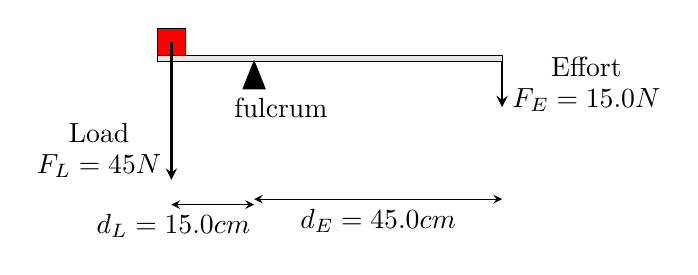
\begin{tikzpicture}[scale=0.7,>=stealth]
        % First class lever
        % rod
        \draw[fill=gray!20] (-0.25,0) rectangle (6,0.1);
        %fulcrum
        \draw[fill=black] (1.3,-0.5) -- (1.7,-0.5) node[below,xshift=2mm] {fulcrum} -- (1.5,0) -- cycle;
        %load
        \draw[fill=red] (-0.25,0.1) rectangle (0.25,0.6);
        \draw[->,thick] (0.0,0.35) -- (0.0,-2.15) node[midway,left,yshift=-0.5cm,align=center] {Load \\\\[-3ex] $F_L = 45N$};
        %effort
        \draw[->,thick] (6,0.0) -- (6,-0.83) node[midway,right,align=center] {Effort \\\\[-3ex] $F_E = 15.0N$};

        % Distance markers
        \draw[<->] (1.5,-2.5) -- (6,-2.5) node[midway,below,align=center] {$d_E = 45.0cm$};
        \draw[<->] (0,-2.6) -- (1.5,-2.6) node[midway,below,xshift=-0.5cm,align=left] {$d_L = 15.0cm$};
    \end{tikzpicture}
\end{minipage}%
\hfill
\begin{minipage}{0.3\textwidth}
    \begin{align*}
        F_E \times d_E &= F_L \times d_L \\
        F_E &= \frac{F_L \times d_L}{d_E} \\
        F_E &= \frac{45 \times 15.0}{45.0} \\
        F_E &= 15.0N
    \end{align*}
\end{minipage}
\pagebreak ~ \newline ~ \newline\refstepcounter{minipagecount}
\noindent{(\theminipagecount)}\quad

\begin{minipage}{0.65\textwidth}
    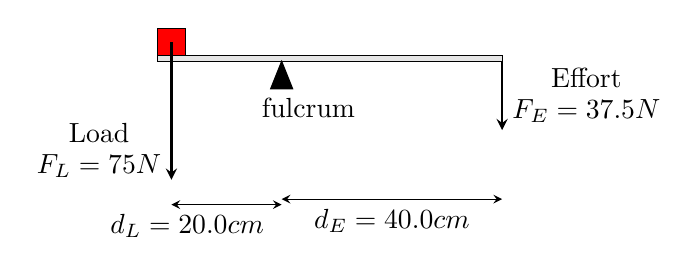
\begin{tikzpicture}[scale=0.7,>=stealth]
        % First class lever
        % rod
        \draw[fill=gray!20] (-0.25,0) rectangle (6,0.1);
        %fulcrum
        \draw[fill=black] (1.8,-0.5) -- (2.2,-0.5) node[below,xshift=2mm] {fulcrum} -- (2.0,0) -- cycle;
        %load
        \draw[fill=red] (-0.25,0.1) rectangle (0.25,0.6);
        \draw[->,thick] (0.0,0.35) -- (0.0,-2.15) node[midway,left,yshift=-0.5cm,align=center] {Load \\\\[-3ex] $F_L = 75N$};
        %effort
        \draw[->,thick] (6,0.0) -- (6,-1.25) node[midway,right,align=center] {Effort \\\\[-3ex] $F_E = 37.5N$};

        % Distance markers
        \draw[<->] (2.0,-2.5) -- (6,-2.5) node[midway,below,align=center] {$d_E = 40.0cm$};
        \draw[<->] (0,-2.6) -- (2.0,-2.6) node[midway,below,xshift=-0.5cm,align=left] {$d_L = 20.0cm$};
    \end{tikzpicture}
\end{minipage}%
\hfill
\begin{minipage}{0.3\textwidth}
    \begin{align*}
        F_E \times d_E &= F_L \times d_L \\
        F_E &= \frac{F_L \times d_L}{d_E} \\
        F_E &= \frac{75 \times 20.0}{40.0} \\
        F_E &= 37.5N
    \end{align*}
\end{minipage}
\refstepcounter{minipagecount}
\noindent{(\theminipagecount)}\quad

\begin{minipage}{0.65\textwidth}
    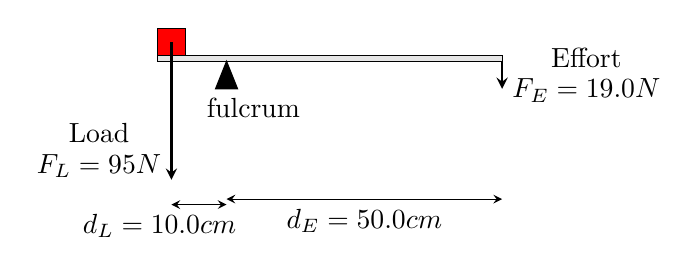
\begin{tikzpicture}[scale=0.7,>=stealth]
        % First class lever
        % rod
        \draw[fill=gray!20] (-0.25,0) rectangle (6,0.1);
        %fulcrum
        \draw[fill=black] (0.8,-0.5) -- (1.2,-0.5) node[below,xshift=2mm] {fulcrum} -- (1.0,0) -- cycle;
        %load
        \draw[fill=red] (-0.25,0.1) rectangle (0.25,0.6);
        \draw[->,thick] (0.0,0.35) -- (0.0,-2.15) node[midway,left,yshift=-0.5cm,align=center] {Load \\\\[-3ex] $F_L = 95N$};
        %effort
        \draw[->,thick] (6,0.0) -- (6,-0.5) node[midway,right,align=center] {Effort \\\\[-3ex] $F_E = 19.0N$};

        % Distance markers
        \draw[<->] (1.0,-2.5) -- (6,-2.5) node[midway,below,align=center] {$d_E = 50.0cm$};
        \draw[<->] (0,-2.6) -- (1.0,-2.6) node[midway,below,xshift=-0.5cm,align=left] {$d_L = 10.0cm$};
    \end{tikzpicture}
\end{minipage}%
\hfill
\begin{minipage}{0.3\textwidth}
    \begin{align*}
        F_E \times d_E &= F_L \times d_L \\
        F_E &= \frac{F_L \times d_L}{d_E} \\
        F_E &= \frac{95 \times 10.0}{50.0} \\
        F_E &= 19.0N
    \end{align*}
\end{minipage}
\refstepcounter{minipagecount}
\noindent{(\theminipagecount)}\quad

\begin{minipage}{0.65\textwidth}
    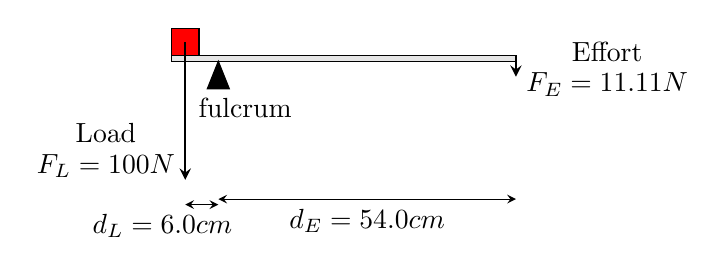
\begin{tikzpicture}[scale=0.7,>=stealth]
        % First class lever
        % rod
        \draw[fill=gray!20] (-0.25,0) rectangle (6,0.1);
        %fulcrum
        \draw[fill=black] (0.4,-0.5) -- (0.8,-0.5) node[below,xshift=2mm] {fulcrum} -- (0.6,0) -- cycle;
        %load
        \draw[fill=red] (-0.25,0.1) rectangle (0.25,0.6);
        \draw[->,thick] (0.0,0.35) -- (0.0,-2.15) node[midway,left,yshift=-0.5cm,align=center] {Load \\\\[-3ex] $F_L = 100N$};
        %effort
        \draw[->,thick] (6,0.0) -- (6,-0.28) node[midway,right,align=center] {Effort \\\\[-3ex] $F_E = 11.11N$};

        % Distance markers
        \draw[<->] (0.6,-2.5) -- (6,-2.5) node[midway,below,align=center] {$d_E = 54.0cm$};
        \draw[<->] (0,-2.6) -- (0.6,-2.6) node[midway,below,xshift=-0.5cm,align=left] {$d_L = 6.0cm$};
    \end{tikzpicture}
\end{minipage}%
\hfill
\begin{minipage}{0.3\textwidth}
    \begin{align*}
        F_E \times d_E &= F_L \times d_L \\
        F_E &= \frac{F_L \times d_L}{d_E} \\
        F_E &= \frac{100 \times 6.0}{54.0} \\
        F_E &= 11.11N
    \end{align*}
\end{minipage}
\refstepcounter{minipagecount}
\noindent{(\theminipagecount)}\quad

\begin{minipage}{0.65\textwidth}
    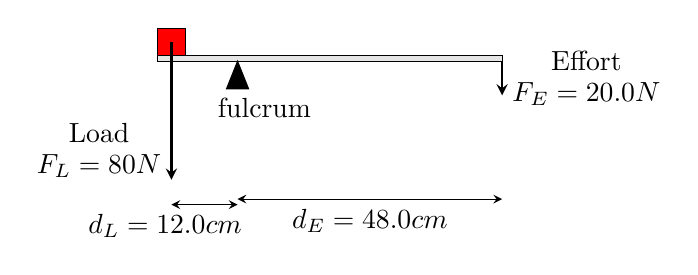
\begin{tikzpicture}[scale=0.7,>=stealth]
        % First class lever
        % rod
        \draw[fill=gray!20] (-0.25,0) rectangle (6,0.1);
        %fulcrum
        \draw[fill=black] (1.0,-0.5) -- (1.4,-0.5) node[below,xshift=2mm] {fulcrum} -- (1.2,0) -- cycle;
        %load
        \draw[fill=red] (-0.25,0.1) rectangle (0.25,0.6);
        \draw[->,thick] (0.0,0.35) -- (0.0,-2.15) node[midway,left,yshift=-0.5cm,align=center] {Load \\\\[-3ex] $F_L = 80N$};
        %effort
        \draw[->,thick] (6,0.0) -- (6,-0.62) node[midway,right,align=center] {Effort \\\\[-3ex] $F_E = 20.0N$};

        % Distance markers
        \draw[<->] (1.2,-2.5) -- (6,-2.5) node[midway,below,align=center] {$d_E = 48.0cm$};
        \draw[<->] (0,-2.6) -- (1.2,-2.6) node[midway,below,xshift=-0.5cm,align=left] {$d_L = 12.0cm$};
    \end{tikzpicture}
\end{minipage}%
\hfill
\begin{minipage}{0.3\textwidth}
    \begin{align*}
        F_E \times d_E &= F_L \times d_L \\
        F_E &= \frac{F_L \times d_L}{d_E} \\
        F_E &= \frac{80 \times 12.0}{48.0} \\
        F_E &= 20.0N
    \end{align*}
\end{minipage}
\refstepcounter{minipagecount}
\noindent{(\theminipagecount)}\quad

\begin{minipage}{0.65\textwidth}
    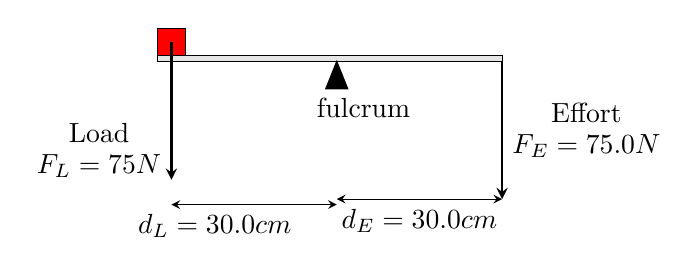
\begin{tikzpicture}[scale=0.7,>=stealth]
        % First class lever
        % rod
        \draw[fill=gray!20] (-0.25,0) rectangle (6,0.1);
        %fulcrum
        \draw[fill=black] (2.8,-0.5) -- (3.2,-0.5) node[below,xshift=2mm] {fulcrum} -- (3.0,0) -- cycle;
        %load
        \draw[fill=red] (-0.25,0.1) rectangle (0.25,0.6);
        \draw[->,thick] (0.0,0.35) -- (0.0,-2.15) node[midway,left,yshift=-0.5cm,align=center] {Load \\\\[-3ex] $F_L = 75N$};
        %effort
        \draw[->,thick] (6,0.0) -- (6,-2.5) node[midway,right,align=center] {Effort \\\\[-3ex] $F_E = 75.0N$};

        % Distance markers
        \draw[<->] (3.0,-2.5) -- (6,-2.5) node[midway,below,align=center] {$d_E = 30.0cm$};
        \draw[<->] (0,-2.6) -- (3.0,-2.6) node[midway,below,xshift=-0.5cm,align=left] {$d_L = 30.0cm$};
    \end{tikzpicture}
\end{minipage}%
\hfill
\begin{minipage}{0.3\textwidth}
    \begin{align*}
        F_E \times d_E &= F_L \times d_L \\
        F_E &= \frac{F_L \times d_L}{d_E} \\
        F_E &= \frac{75 \times 30.0}{30.0} \\
        F_E &= 75.0N
    \end{align*}
\end{minipage}


\end{document}
